% ------------- DEFINITION DU DOCUMENT -------------

\documentclass[12pt, oneside]{report}
% Types de documents possibles : book, article, report, slides
% Options pour la police du document et sa mise en page globale. Se référer au manuel pour liste exhaustive.


% ------------- GESTION DES LANGUES -------------

\usepackage[english]{babel}
\usepackage[T1]{fontenc} % Ne pas utiliser si XeTeX ou LuaTeX
\usepackage[utf8]{inputenc} % Ne pas utiliser si XeTeX ou LuaTeX

% ------------- MISE EN PAGE GLOBALE -------------

% Package gérant la taille des marges. Pour plus de détails sur la mise en page, utiliser \layout
\usepackage[top=3.0cm, bottom=3.0cm, left=2.5cm, right=2.5cm]{geometry}

% Gestion des entêtes/pieds (plain : pieds, headings : en-tête, empty : rien; appliquer sur une page, \thispagestyle{})
\pagestyle{plain}
% Gestion du pack de police utilisé pour le document
\usepackage{lmodern}

%¨Police Personnalisée /!\ A Utiliser avec le moteur XeTex ou LuaTex
%\usepackage{fontspec} 
%\setmainfont{Vinci_Serif_Regular.otf}[
%BoldFont = Vinci_Serif_Bold.otf ,
%ItalicFont = Vinci_Serif_Italic.otf ,
%BoldItalicFont = Vinci_Serif_Bold_Italic.otf ]

% Mise des \todo{}
\usepackage[colorinlistoftodos]{todonotes}


% A décommenter pour ne plus afficher le header des chapitres
%\usepackage{titlesec}
%\titleformat{\chapter}
%  {\Large\bfseries} % format
%  {}                % label
%  {0pt}             % sep
%  {\huge}           % before-code


% ------------- PACKAGE DE MISE EN PAGE -------------

% Package pour la gestion des interlignes (déclaration de type environnement; onehalfspace, doublespace...)
\usepackage{setspace}
% Pour \st (barrer) et \ul (souligner)
\usepackage{soul}
% Pour colorier le texte
\usepackage{color}
% Pour la mise en page de code source
\usepackage{listings}
% Pour les indices (\textsubscript{})
\usepackage{subscript}
% Pour utiliser les liens : \url{ } 
\usepackage{hyperref}

\usepackage{subfig}


% ------------- PACKAGE MATH -------------

% Pour ouvrir l'environnement math : $, $$, \begin{math}, et \begin{equation}

\usepackage{amsmath}
\usepackage{amssymb}
\usepackage{mathrsfs}


% ------------- INSERTION IMAGES -------------

\usepackage{graphicx}

% Inclure les images avec \includegraphics{chemin}
% Options : height=, width= ou scale=, angle=

% Environnements flottants : \begin{figure}[placement] à coupler avec une environnement d'alignement
% Options de placement : t (top), h (ici), b (bas), ...

% légendes : \caption{} à placer à la suite de l'environnement center, dans l'environnement flottant

% \clearpage crée une nouvelle page avec mise en place préalable des flottants


% ------------- TABLEAUX -------------

% Créer un tableau avec \begin{tabular}{cc} avec en 2ème accolade les alignements et le nombre de colonnes
% Options d'alignement : c, r et l, et p[largeur]
% Séparateurs : | et @{<separateur>} permettent de spécifier la position des séparateurs verticaux (a placer dans la 2ème accolade). \hline crée une ligne horizontale 

% & permet de séparer les cellules sur la même ligne. \\ crée une nouvelle ligne.

% Pour utiliser \backslashbox{}{}
\usepackage{diagbox}

% Pour créer une table : \begin{table}. Se comporte comme un flottant.


% ------------- GESTION DU CODE SOURCE ET ALGO -------------

\lstset{
language=C++,        		% choix du langage (C, C++, Java, PHP, SQL, XML, HTML, ...). Peut se choisir localement avec language=
basicstyle=\footnotesize,       % taille de la police du code
numbers=left,                   % placer le numéro de chaque ligne à gauche (left)
numberstyle=\normalsize,        % taille de la police des numéros
numbersep=10pt,                  % distance entre le code et sa numérotation
backgroundcolor=\color{white},  % couleur du fond 
}
% S'utilise avec l'environnement \begin{lstlisting}[frame=one] et \lstinputlisting{fichier_source}

\usepackage[linesnumbered]{algorithm2e}


% ------------- TITRE -------------

% Création de la page de titre avec \maketitle


% ------------- TABLE DES MATIERES -------------

% Création de la table des matières avec \tableofcontents

% Redéfinit le titre de la table des matières
\AtBeginDocument{\renewcommand{\contentsname}{Table des Matières}}
% Indique les éléments à inclure : -1 correspond aux parties, 5 aux sous-paragraphes
\setcounter{tocdepth}{3}


% ------------- CORPS DU DOCUMENT -------------

\begin{document}

\begin{center}
\Large{
\textbf{DH2323 Project Specification : \\ Implementing a Pathtracer}
} 
\medskip
\small{\\Jonathan Guichard}
\end{center}

\bigskip

\section*{Background}

\paragraph{}Pathtracing is a computer graphics method of rendering images of three-dimensional scenes such that the global illumination is faithful to the reality. It "naturally" simulates many effects, such as shoft shadows, ambient occlusion and indirect lighting, that otherwise have to be coded into rendering methods like raytracing. The fundamental principle allowing this consists of casting light rays starting from the camera, then recursively casting new random rays in order to determine the color of the hit area, by using the rendering equation. \\
This method can produce photorealistic results as shown below, but also requires a long rendering time in order to obtain a noiseless image - as a great number of rays must be traced. Pathtracing plays a significant role in the movie industry and is often used to generate reference images used to judge other rendering methods.

\medskip

\begin{figure}[h]
  \centering
    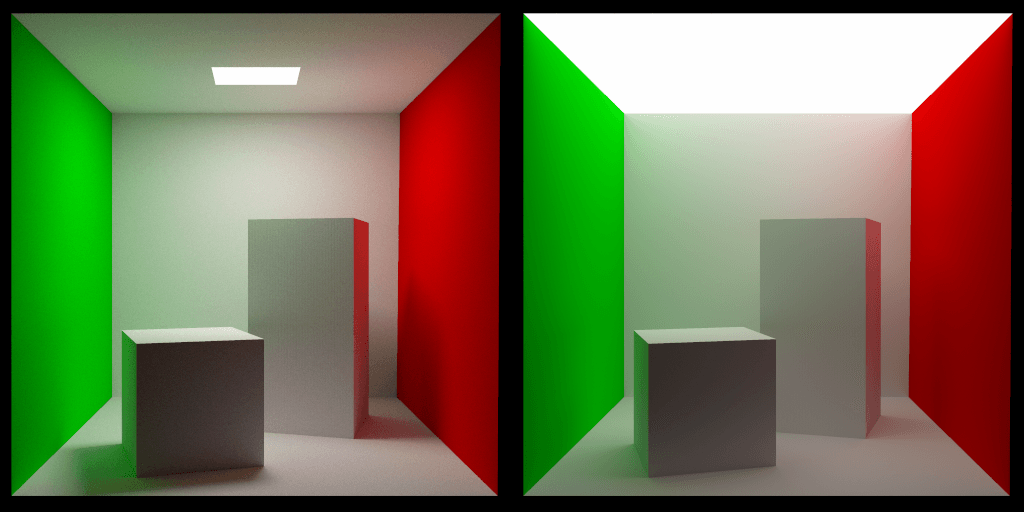
\includegraphics[scale=0.4]{example.png}
    \caption{Example of cornell box rendered with pathtracing}
\end{figure}

\section*{Specification}

\paragraph{}The goal of this project is to implement a very simple pathtracer, capable of rendering a scene of the same complexity as the one used in labs 2 and 3 of the rendering track. \\
In other words, the pathtracer we implement must be capable of rendering a simple Cornell Box with a fixed surface light source on the roof, of variable size and emitted color. The camera has a fixed position and can not rotate, and we consider all the objects present in the scene to be made of the same material and to be ideally diffuse. We do not render any complex materials and phenomenons that would require some specific handling, such as water, glass, specular surfaces or caustics, to only name a few. \\ Time permitting, more complex features might be added on top of this initial kernel.

\paragraph{}The objective of this project is to be able to render a cornell box and to compare pathtracing to the two other different rendering methods implemented during the labs of the rendering track. We also want to explore the effect of the number of samples (i.e. the number of rays being recursively traced) and the maximum recursion depth on the final rendered image.

\nocite{*}


% non-implementation goals : exploring the effect of the parameters (depth and sampling) on different images, trying to explain why we see this.


\end{document}
